During Run 2, the muon system of CMS was composed of three sub-detectors whose information was combined in order to optimize muon reconstruction. These three sub-detectors are the Cathode Strip Chambers, the Resistive Plate Chambers, and the Drift Tubes described in Sections \ref{sec:CSC}, \ref{sec:RPC} and \ref{sec:DT} respectively. During LS2, the installation of a new muon system called the Gas Electron Multiplier (GEM) was completed in order to improve muon identification through the addition of additional measurements. This new sub-detector is currently being commissioning for LHC Run 3. A diagram including all CMS muon subsystems, as of the beginning of LHC Run 3, is shown in Figure \ref{fig:MuonSystem}.

\begin{figure}[H]
    \centering
    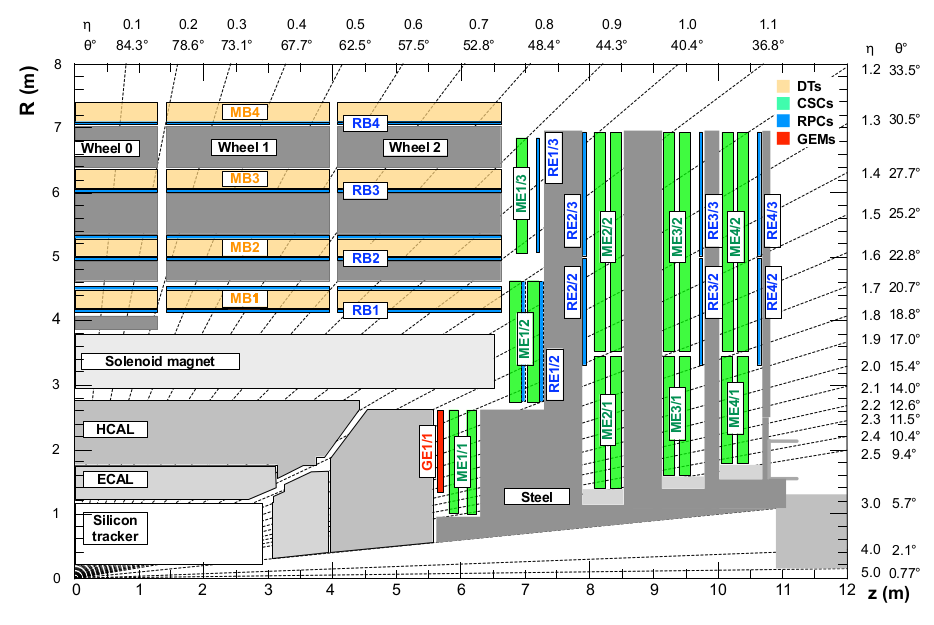
\includegraphics[width=0.7\textwidth]{Images/CMS/Muons/MuonSystem.png}
    \caption{CMS muon system at the start of LHC Run 3.}
    \label{fig:MuonSystem}
\end{figure}

% Probably going to need all of these references later.
% https://cds.cern.ch/record/2665948/
% arXiv:1903.02186v2
% https://arxiv.org/pdf/1804.04528.pdf
% https://twiki.cern.ch/twiki/bin/view/CMSPublic/MuonDPGResults

\subsubsection{Cathode Strip Chambers}
% public reference 
% https://indico.cern.ch/event/782953/contributions/3482451/attachments/1888308/3114226/20190801-DPF2019-ALW-final.pdf
% https://inspirehep.net/literature/1790595
% https://cms.cern/detector/detecting-muons/cathode-strip-chambers

% https://indico.cern.ch/event/663474/contributions/3060096/attachments/1681230/2701095/ICNFP2018_Overview_CMS_performance.pdf
% https://twiki.cern.ch/twiki/bin/view/CMSPublic/MuonDPGPublic160729
% https://twiki.cern.ch/twiki/bin/view/CMSPublic/MuonDPGResults

The CMS Cathode Strip Chambers (CSC) are a group of 540 gas ionization chambers located in the CMS endcaps. The CSC cavities are filled with a gas mixture composed of Ar, $CO_{2}$ and $CF_{4}$, and detect muons via ionization of this gas mixture. A diagram showing a CSC and its mechanism for muon detection is shown in Figure \ref{fig:CSC_Diagram}. 

\begin{figure}[H]
    \centering
    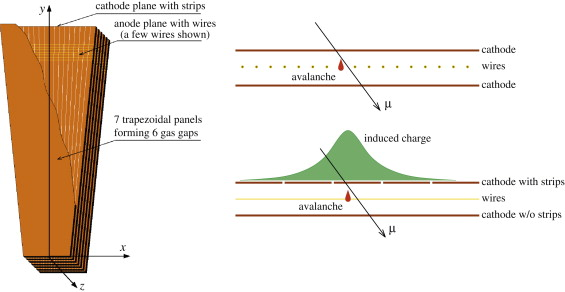
\includegraphics[width=0.7\textwidth]{Images/CMS/Muons/CSC/CSC_image.jpg}
    \caption{Muon detection in the CMS CSCs}
    \label{fig:CSC_Diagram}
\end{figure}

When an energetic muon from an LHC collision strikes a CSC, it knocks the electrons off of the atoms making up the CSC gas mixture. These electrons are forced to the anodes (positive ions forced to the cathodes) due to the presence of an electric potential, which produces an avalanche of electrons and thus a net charge.

The CSCs performed extremely well during Run 2, with an average segment reconstruction efficiency around 97\%, shown for the 2016 data taking year in Figure \ref{fig:CSC_2016SegHitEff}.

\begin{figure}[H]
    \centering
    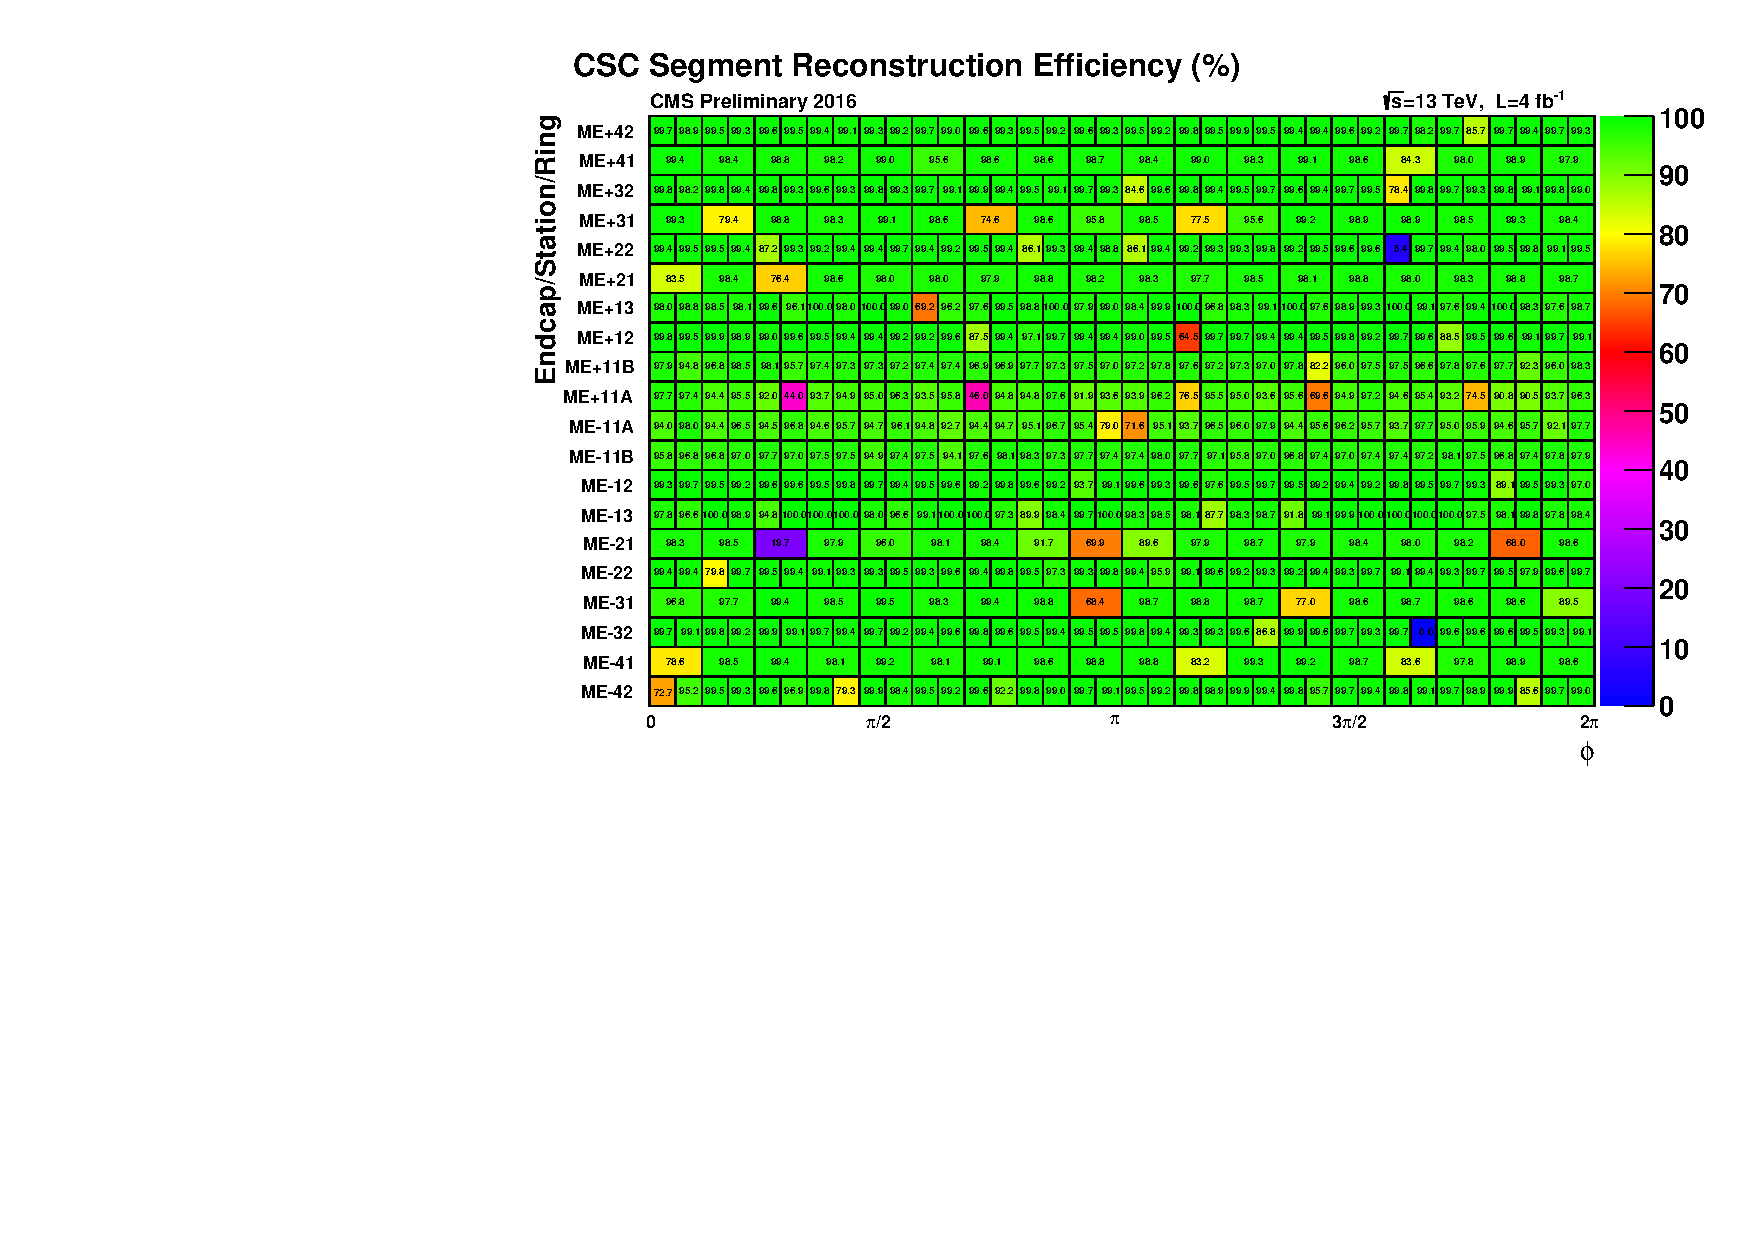
\includegraphics[width=0.85\textwidth]{Images/CMS/Muons/CSC/seg_eff_Muon_JSON_June22all_chambers_noErr.pdf}
    \caption{2016 CSC segment reconstruction efficiency.}
    \label{fig:CSC_2016SegHitEff}
\end{figure} \label{sec:CSC}

\subsubsection{Resistive Plate Chambers}
% http://cds.cern.ch/record/2801878/files/document.pdf?version=1
% https://iopscience.iop.org/article/10.1088/1748-0221/16/04/C04004
% https://twiki.cern.ch/twiki/bin/view/Main/EndcapReshufflingRpc

The CMS Resistive Plate Chambers (RPCs) are a group of 1056 chambers placed in both the CMS barrel and endcap sections for muon detection, filled with a gas mixture of $C_{2}H_{2}F_{4}$, $C_{4}H_{10}$ and $SF_{6}$. In a fashion similar to the CSCs, the RPCs detect muons via direct ionization of its gaseous mixture. The layout of an RPC module is shown in Figure \ref{fig:RPC_Schema}. 

\begin{figure}[H]
    \centering
    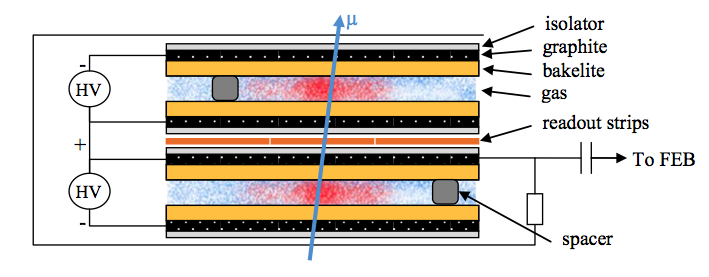
\includegraphics[width=0.9\textwidth]{Images/CMS/Muons/RPC/RPC_Schema.png}
    \caption{RPC schematic.}
    \label{fig:RPC_Schema}
\end{figure}

The idea behind the geometry of an RPC chamber is to have readout strips in the center, with gaseous chambers located on either side. 

Like the CSCs, throughout Run 2 the RPCs maintained excellent hit efficiency, as shown separately for the barrel and endcap portions in Figures \ref{fig:RPC_Barrel_Eff} and \ref{fig:RPC_Endcap_Eff}. 

\begin{figure}[H]
    \centering
    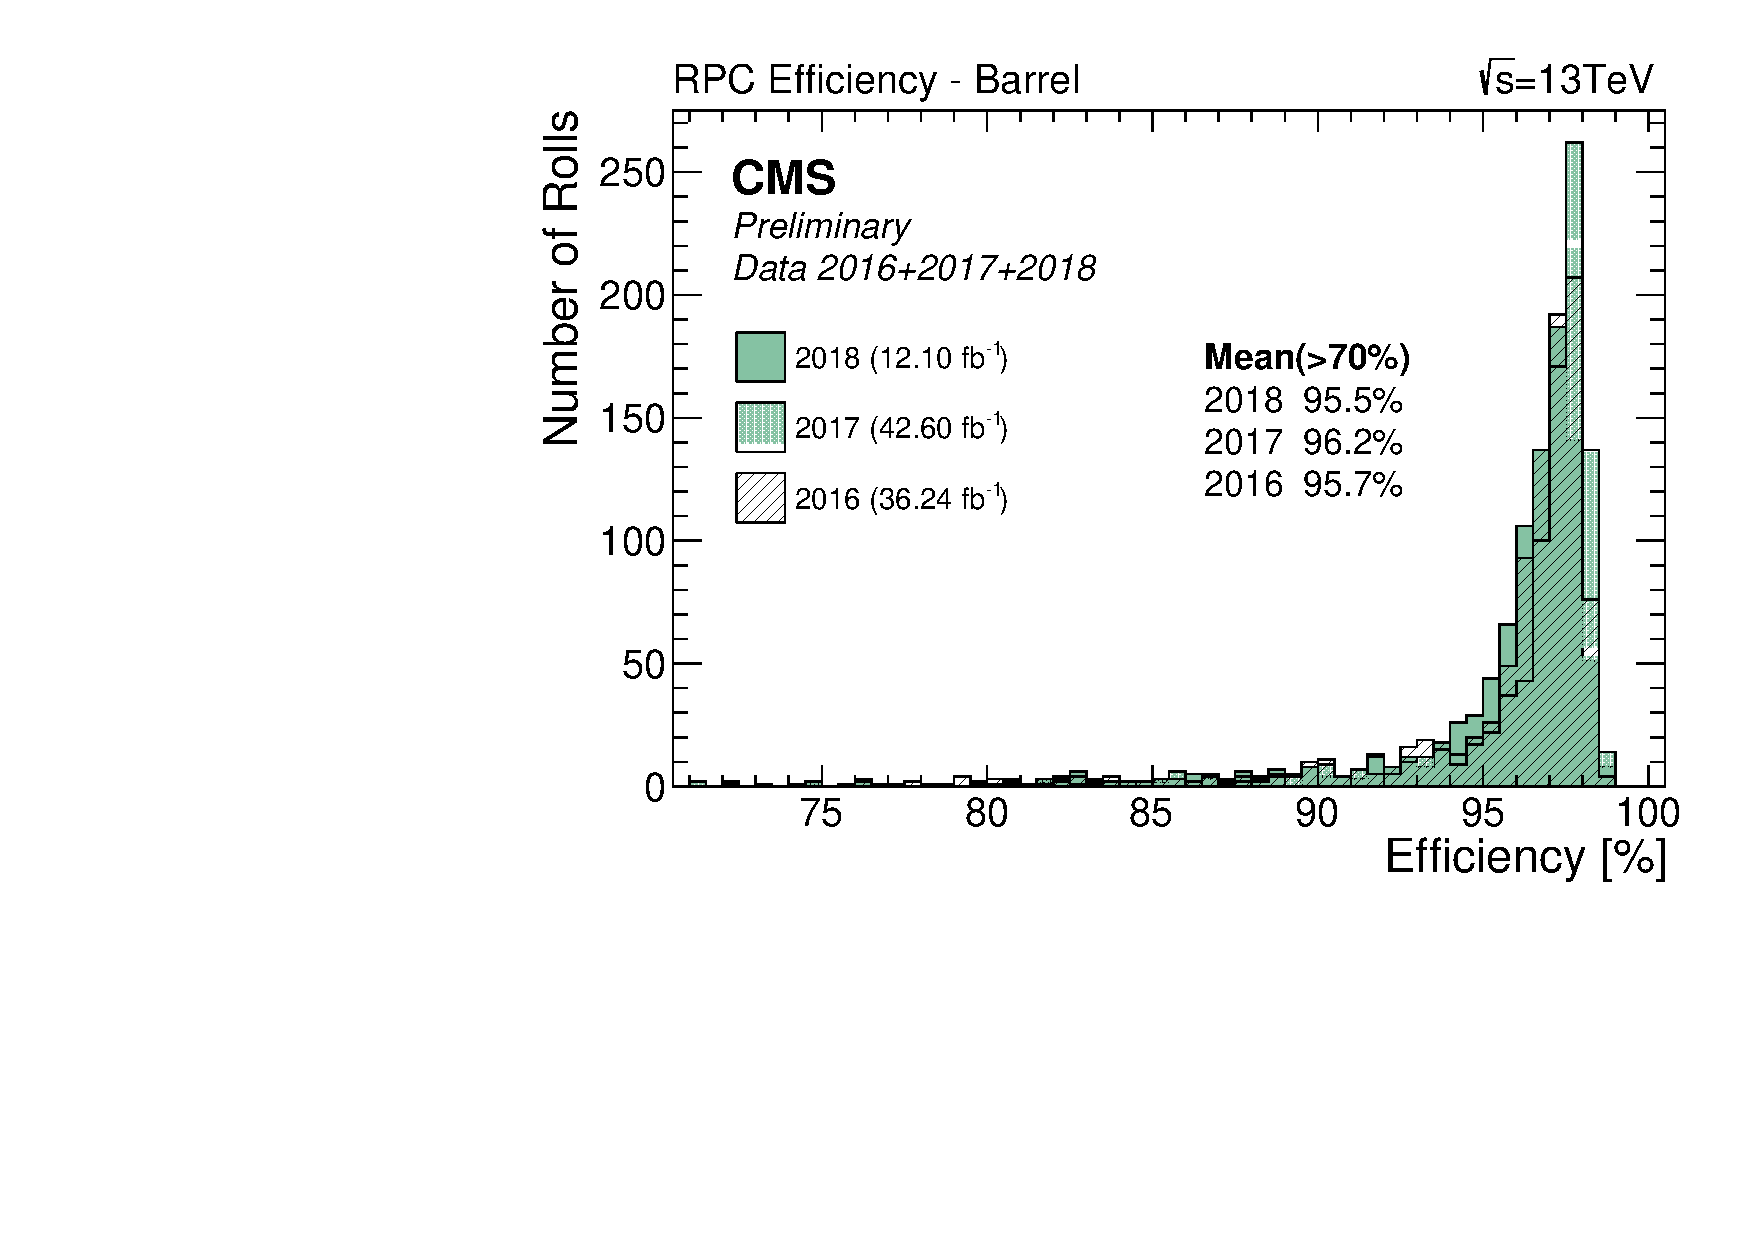
\includegraphics[width=0.7\textwidth]{Images/CMS/Muons/RPC/RPC_EffCmpBarrel.pdf}
    \caption{RPC barrel efficiency during LHC Run 2.}
    \label{fig:RPC_Barrel_Eff}
\end{figure}

\begin{figure}[H]
    \centering
    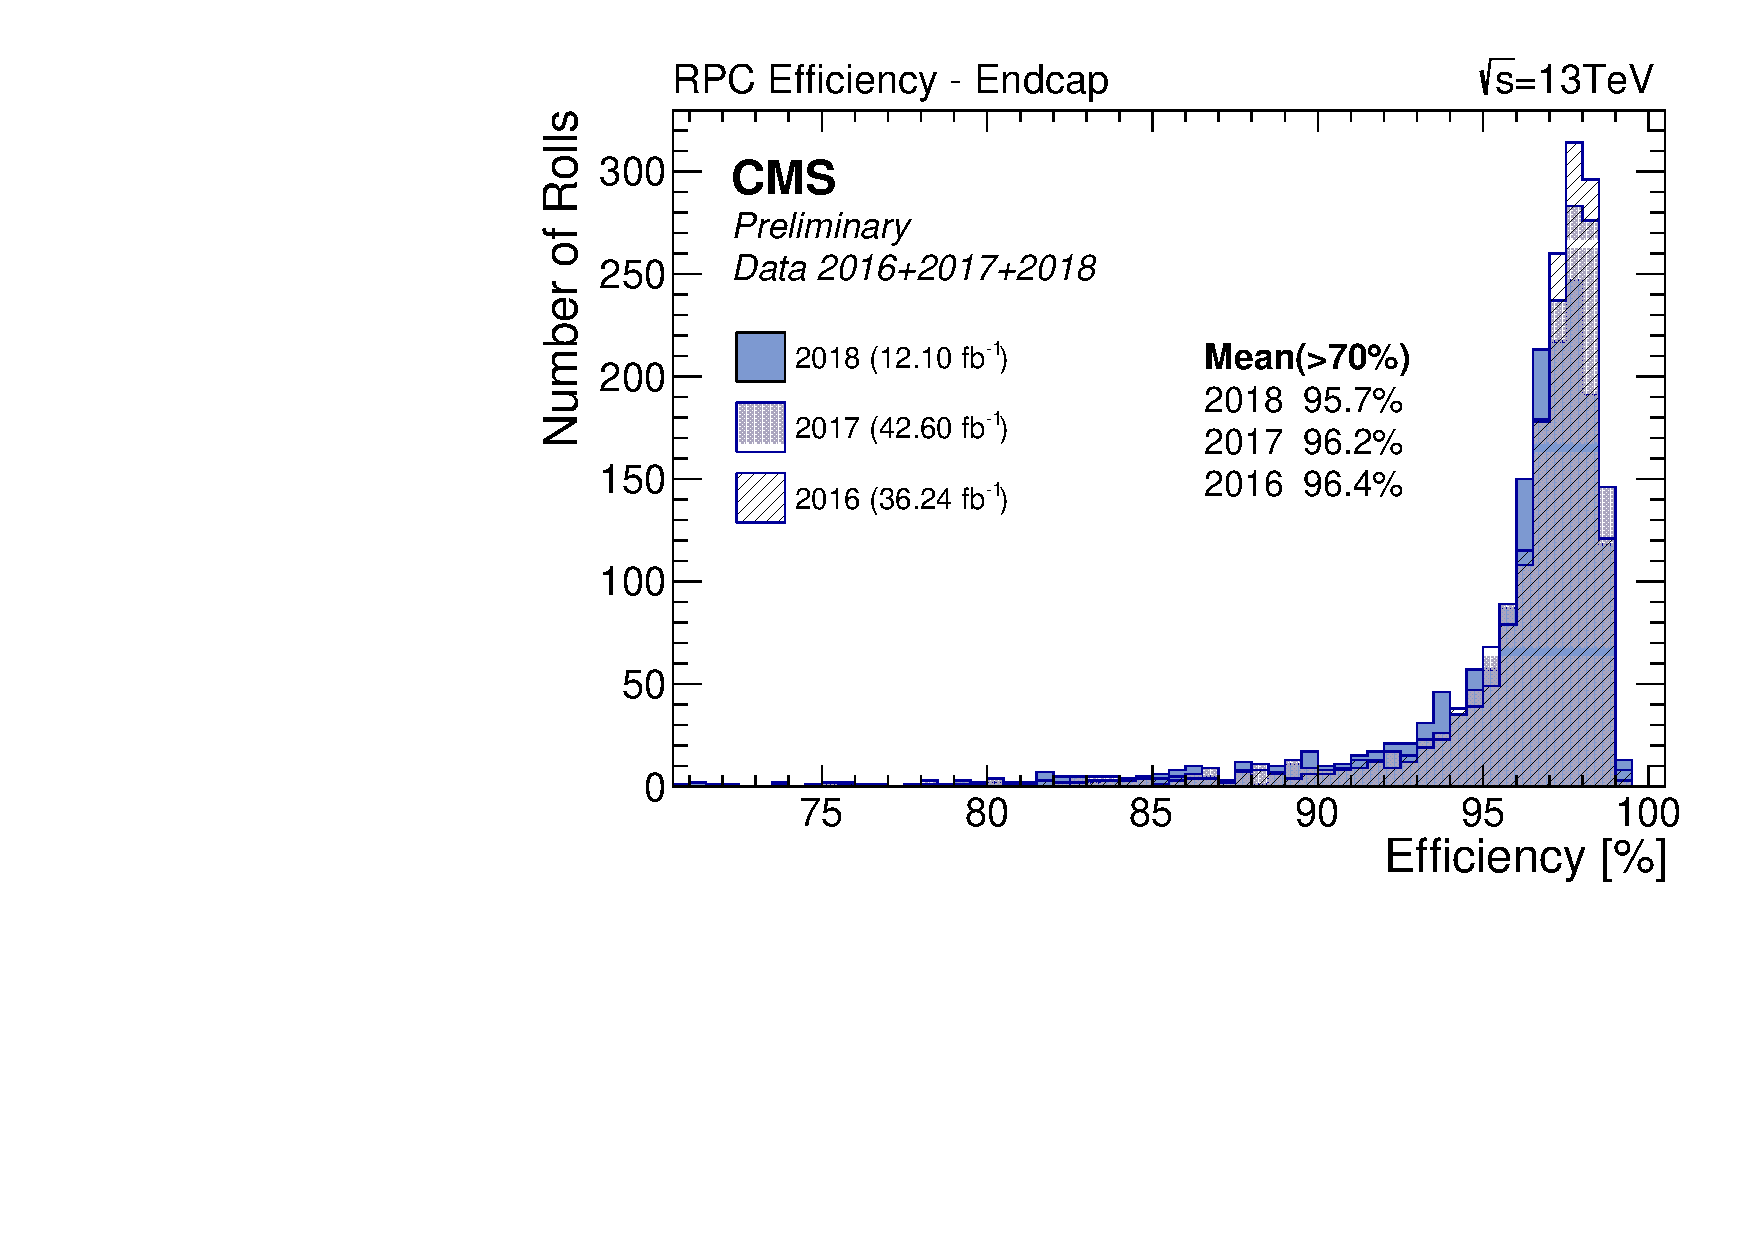
\includegraphics[width=0.7\textwidth]{Images/CMS/Muons/RPC/RPC_EffCmpEndcap.pdf}
    \caption{RPC endcap efficiency during LHC Run 2.}
    \label{fig:RPC_Endcap_Eff}
\end{figure}

 \label{sec:RPC}

\subsubsection{Drift Tubes}
The Drift Tubes (DTs) are a CMS muon system located exclusively in the barrel portion of CMS. They function in a similar way to the CSCs and RPCs, as they detect muons via the direct ionization of a gaseous mixture. A diagram of a DT is shown in Figure \ref{fig:DT_Diagram}. 

\begin{figure}[H]
    \centering
    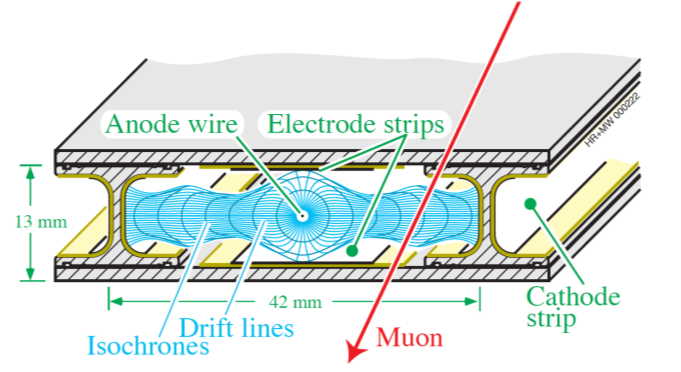
\includegraphics[width=0.7\textwidth]{Images/CMS/Muons/DT/DT_diagram.png}
    \caption{Drift tube diagram}
    \label{fig:DT_Diagram}
\end{figure}

 \label{sec:DT}

% \subsubsection{Gas Electron Multiplier}
% The Gas Electron Multipliers (GEMs) are a new CMS subsystem being installed during LS2 and to operate as a part of CMS during LHC Run 3. 

% https://cds.cern.ch/record/2641471/plots \label{sec:GEM}